\documentclass[11pt]{article}

% Packages
\usepackage[margin=1in]{geometry}
\usepackage[utf8]{inputenc}
\usepackage[T1]{fontenc}
\usepackage{lmodern}
\usepackage{amsmath}
\usepackage{graphicx}
\usepackage{booktabs}
\usepackage{float}
\usepackage{caption}
\usepackage{hyperref}

% Generated figures are in figures/
\graphicspath{{../figures/}}

\title{Project Report: TF-IDF Analysis of Evolution and Ethics Texts}
\author{Lukas Anell}
\date{September 2026}

\begin{document}
\maketitle


\section{Summary}
% Overview of the investigation, findings, and limitations


\section{Introduction}
% Context behind the 5 books, the problem being addressed, my goals, etc.

\begin{table}[H]
	\centering
	\begin{tabular}{llll}
		\toprule
		ID    & Title                    & Author          & Role in comparison \\
		\midrule
		1228  & On the Origin of Species & Charles Darwin  & [ ]                \\
		2300  & The Descent of Man       & Charles Darwin  & [ ]                \\
		2940  & Evolution and Ethics     & T.\,H.\ Huxley  & [ ]                \\
		46129 & The Data of Ethics       & Herbert Spencer & [ ]                \\
		4341  & Mutual Aid               & Peter Kropotkin & [ ]                \\
		\bottomrule
	\end{tabular}
	\caption{Documents analyzed (Project Gutenberg's plaintext editions).}
	\label{tab:books}
\end{table}


\section{Methodology}
% What I did and why

\subsection{Data Collection}
% Downloading from Gutenberg, folder structure

\subsection{Text Cleaning and Trimming}
% Removing boilerplate, trimming the Huxley work, frontmatters/tables of contents

\subsection{Normalization and Tokenization}
% Casefolding, NFC, fix for "--" showing up, punctuation removal, stopword removal, single-character and numeric filters, word-document table

\subsection{Vectorization and TF-IDF}
Term frequency, inverse document frequency, and TF-IDF were computed with
pandas and numpy following the definitions in the project handout:
\begin{align}
	\mathrm{tf}(t, d)       & = \frac{f(t, d)}{\sum_{t' \in d}{f(t', d)}}  \\
	\mathrm{idf}(t, D)      & = \log\!\left(\frac{N_D}{1 + n_t}\right)     \\
	\mathrm{tfidf}(t, d, D) & = \mathrm{tf}(t, d) \cdot \mathrm{idf}(t, D)
\end{align}
% Explain how each step was implemented
% Note that numpy.log is base e

\subsection{Document Comparison}
% Reshaping DataFrames to wide and cosine similarity
\begin{equation}
	\cos(\mathbf{a}, \mathbf{b}) = \frac{\mathbf{a} \cdot \mathbf{b}}{\lVert \mathbf{a} \rVert \, \lVert \mathbf{b} \rVert}
\end{equation}


\section{Results}
% Tie findings back to the goals in the introduction
% Explain what the findings mean

\subsection{Vocabulary}
% Vocabulary size, genre-related words, effect of stopword removal on the data

\subsection{Term Frequency}
% Significance of sorted TF values

\subsection{Inverse Document Frequency}
% Significance of IDF values
% lowest vs. highest, and negative ones

\subsection{TF-IDF}
% Highest TF-IDF term per document and what it means

\begin{figure}[htbp]
	\centering
	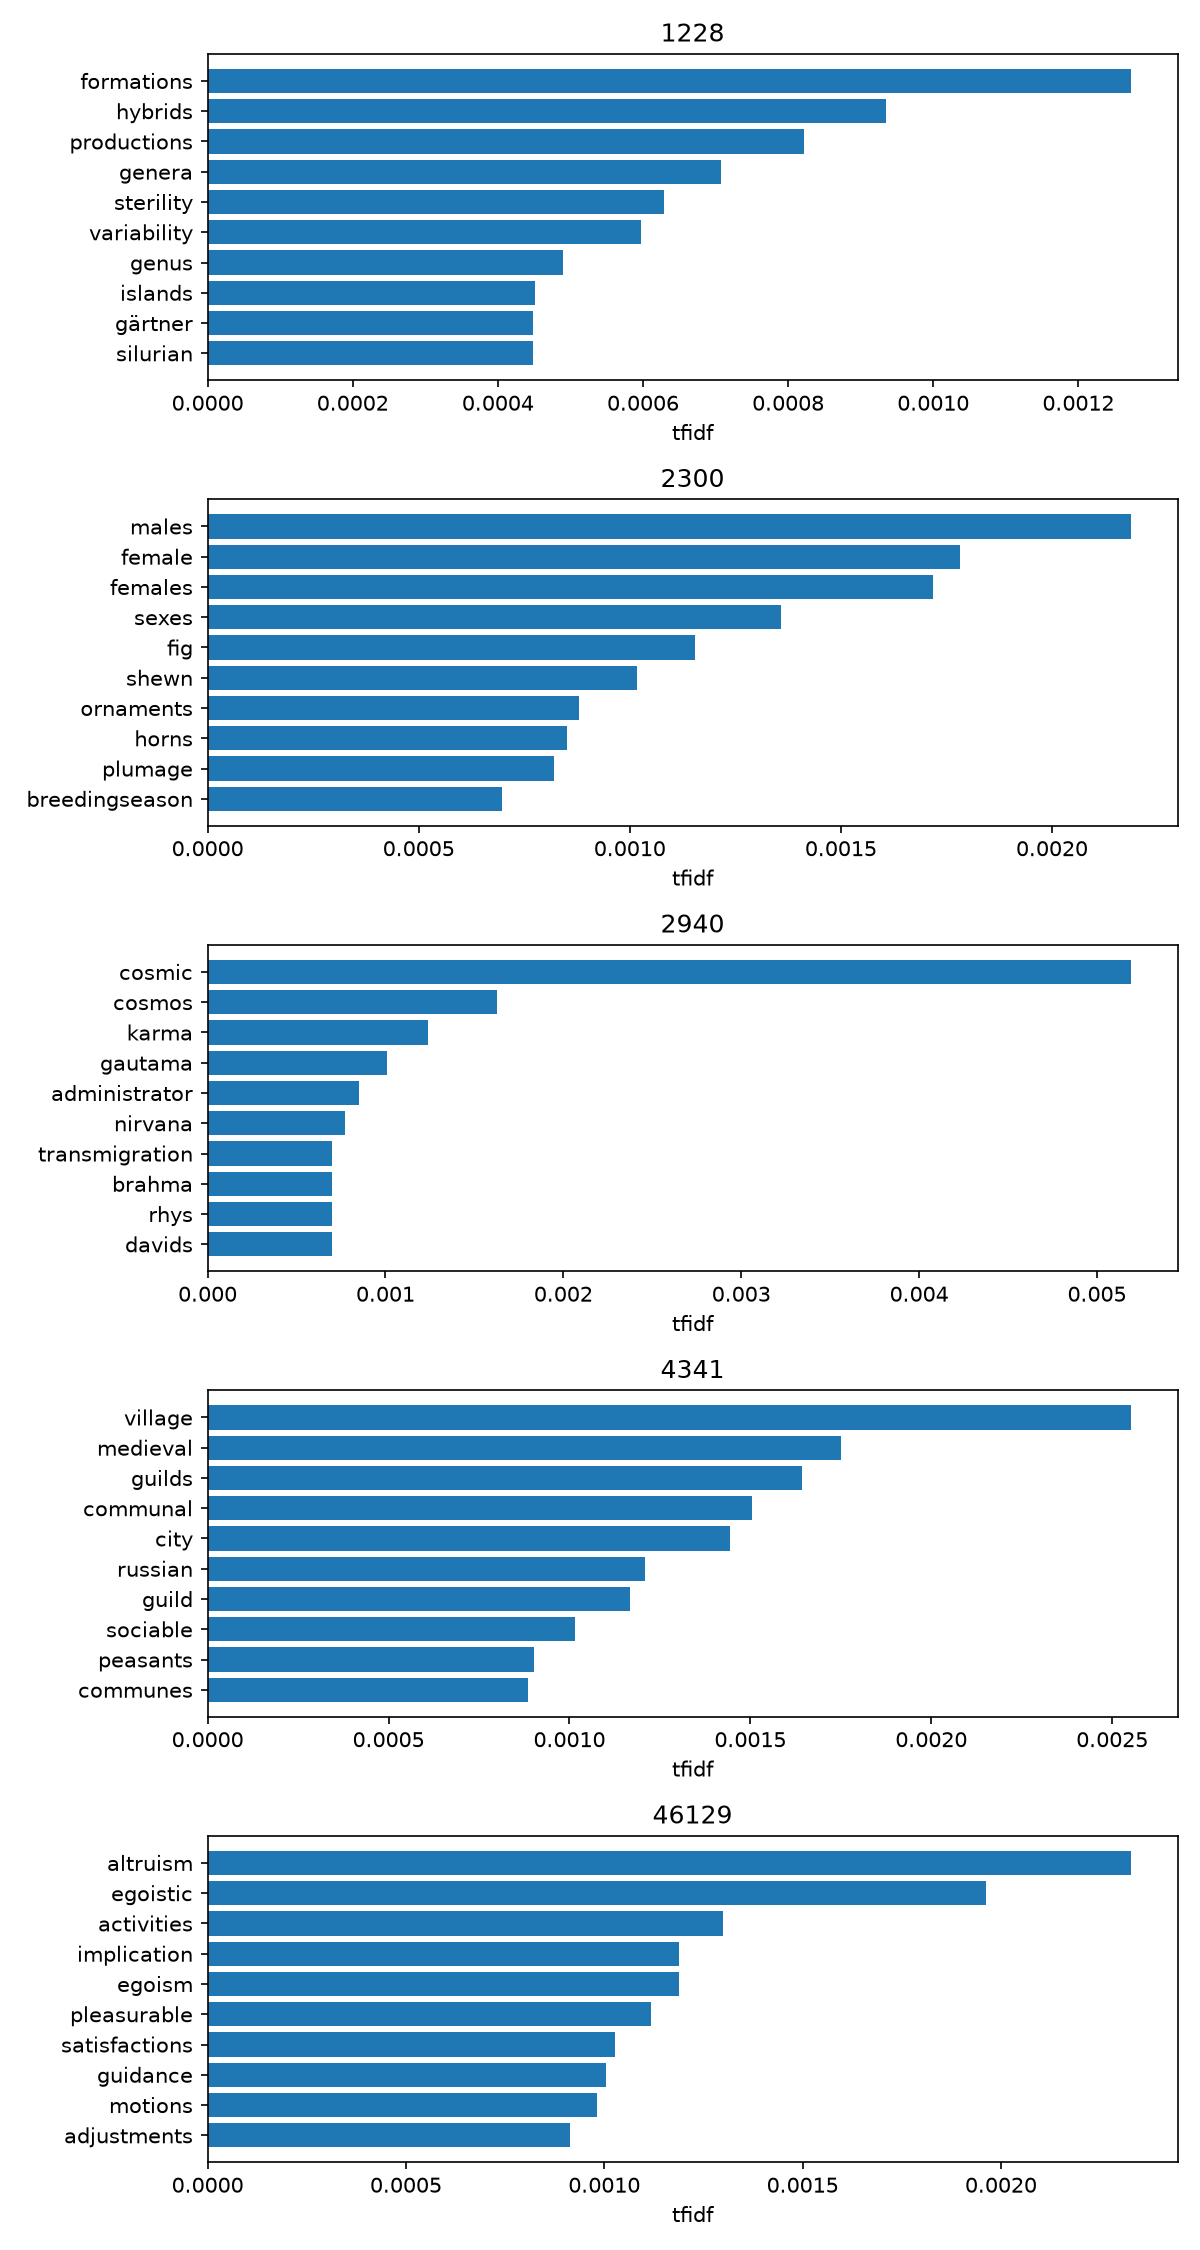
\includegraphics[width=\linewidth,height=0.8\textheight,keepaspectratio]{top_tfidf_terms.png}
	\caption{Top ten TF-IDF terms for each book.}
	\label{fig:top-tfidf}
\end{figure}

\subsection{Document Similarity}
% Talk about the cosine similarity between books
% Does the spectrum between science and ethics show up?

\begin{figure}[H]
	\centering
	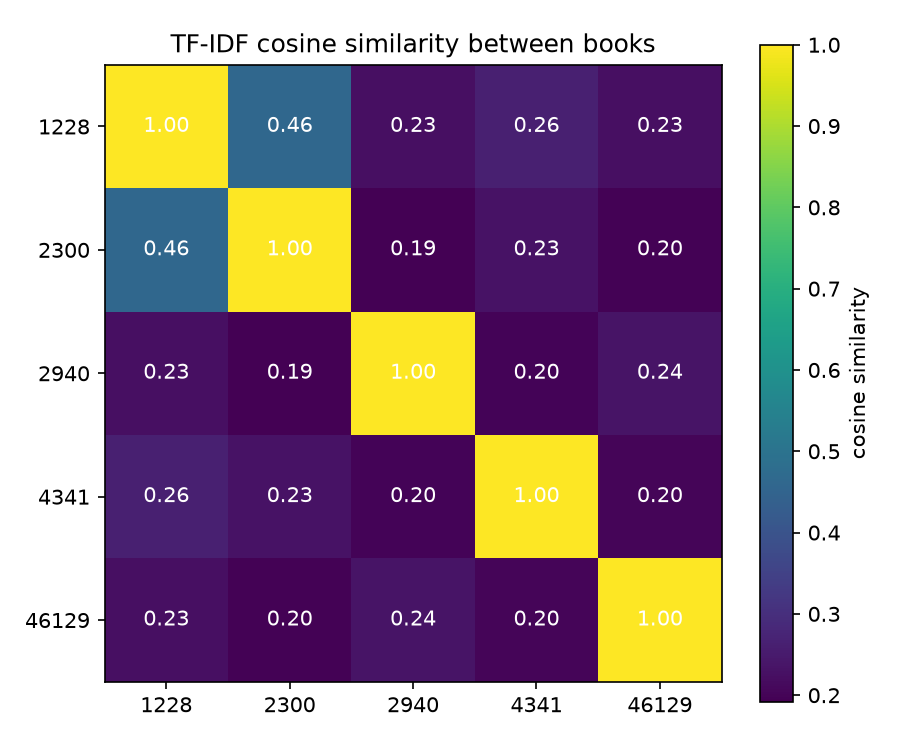
\includegraphics[width=0.6\linewidth]{tfidf_similarity.png}
	\caption{Cosine similarity between the books' TF-IDF vectors.}
	\label{fig:similarity}
\end{figure}

\subsection{Exploration}
% Maybe do tf-only similarity, bigrams, or extra books?


\section{Conclusion}
% Restate problem and claim
% Talk about why my results support my claim
% Include call for action for further research and projects


\section{Reflection}
% Reflect on experience while completing analysis

\subsection{Something I Understand Differently Now}

\subsection{A Decision I Made}

\subsection{A Moment of Uncertainty}

\subsection{Looking Back}


\bibliographystyle{plain}
\bibliography{references}
\nocite{*}

\end{document}
